%2785
\newpage
\subsection{例題4-14 照度センサーを使ったゲームを遊んでみよう}

\begin{description}
    \item \textgt{\bf 考え方}
\end{description}


アイデア\ruby{次第}{し|だい}で、キーボードだけでなく、センサー\ruby{類}{るい}を使ってゲームのようにすることができます。

光センサーを使ったゲームを動かしてみましょう。


スクリプトエディタの、ファイル→「開く」メニューから「catch.hsp」を読み込んで実行してみてください。


\begin{description}
    \item \textgt{\bf 例題4-14 答え}
\end{description}

センサーボードの光センサーから得た値を使って絵を動かしています。光センサーを手で\ruby{覆}{おお}ったり、\ruby{離}{はな}したりしてどうなるか確認してみましょう。

光センサーが暗くなった時には、キャラクターが左に移動します。光センサーが明るくなった時には、キャラクターが右に移動します。


\begin{figure}[H]
    \begin{center}
      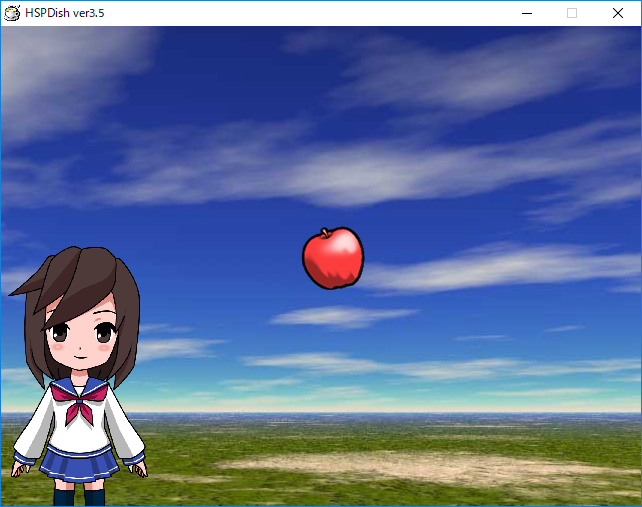
\includegraphics[keepaspectratio,width=11.269cm,height=8.89cm]{text04-img/text04-img041.png}
      \caption{catch.hspの実行画面}
    \end{center}
    \label{fig:prog_menu}
\end{figure}

うまくキャラクターを移動させて、上から落ちてくるリンゴをキャッチしてみましょう。

これは、いままでの応用ですが、センサーと動きのある画面を組み合わせるだけでも、面白いものが作れるはずです。gpio命令で、LEDを光らせたり、スイッチを読み取ったりということと、変数・条件判断を組み合わせれば、さらに\ruby{応用範囲}{おう|よう|はん|い}が広がります。

%2844












